
%\documentclass[./main.tex(path of main file)]{subfiles}
\documentclass[10pt]{article}
\usepackage{amsmath}
\DeclareMathOperator*{\argmin}{arg\,min} % thin space, limits underneath in displays
\DeclareMathOperator*{\argmax}{arg\,max} % thin space, limits underneath in displays
\newtheorem{thm}{Theorem}
\usepackage{amssymb}
\usepackage{amsfonts}
\usepackage{mathrsfs}
\usepackage{bm}
\usepackage{indentfirst}
\setlength{\parindent}{0em}
\usepackage[margin=1in]{geometry}
\usepackage{graphicx}
\usepackage{setspace}
\doublespacing
\usepackage[flushleft]{threeparttable}
\usepackage{booktabs,caption}
\usepackage{float}
\usepackage[sort,comma]{natbib}
\usepackage[hidelinks]{hyperref}
\usepackage{booktabs}
\usepackage{multirow}

\usepackage{import}
\usepackage{xifthen}
\usepackage{pdfpages}
\usepackage{transparent}
\usepackage{subfiles}
\usepackage{blindtext}

\newcommand{\incfig}[1]{%
\def\svgwidth{\columnwidth}
\import{./figures/}{#1.pdf_tex}
}




\title{}
\author{}
\date{}


\begin{document}
%\maketitle



\section{Why the sign of coef is different from what we see in a scatter plot?}



\begin{figure}[H]
\center{
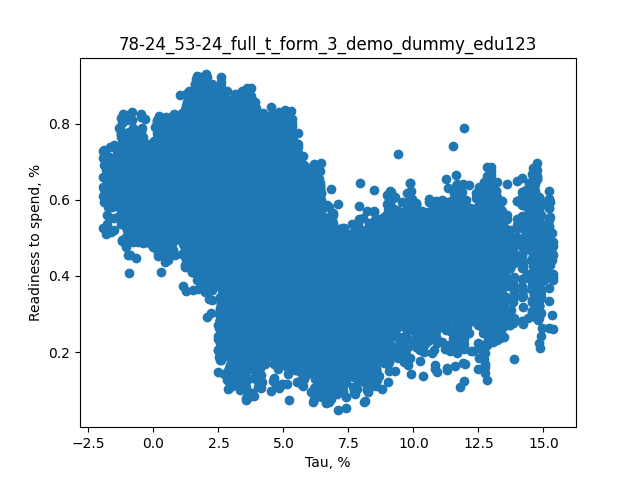
\includegraphics[scale =.7 ]  {./figures/scatter_plot_all_periods.png}
}
\caption{}
\label{fig:scatter_all}
\end{figure}


\begin{figure}[H]
\center{
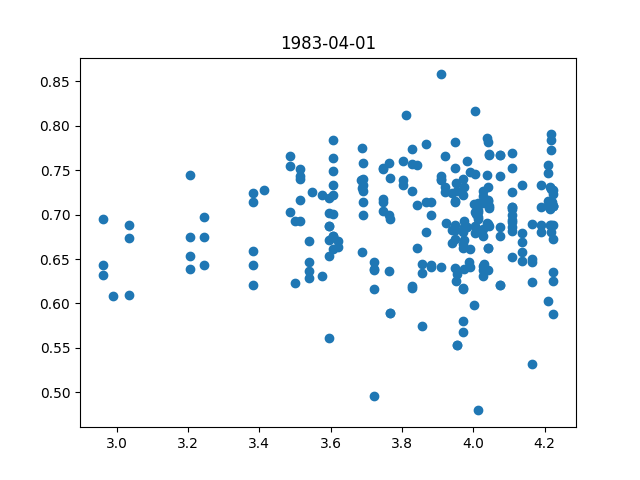
\includegraphics[scale =.5 ]  {./figures/scatter_plot_one_period_high_y.png}
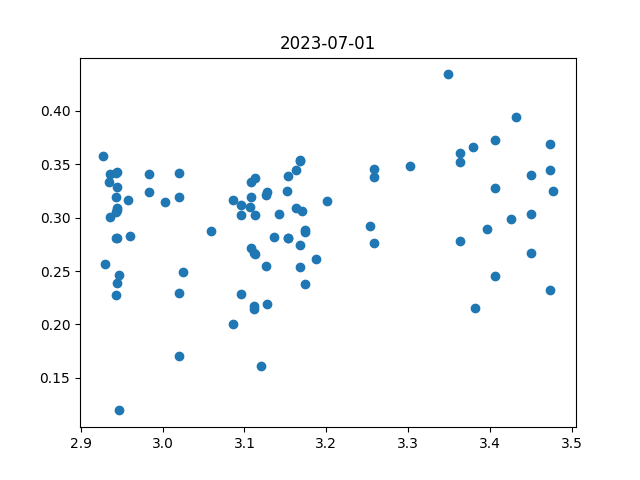
\includegraphics[scale =.5 ]  {./figures/scatter_plot_one_period_low_y.png}
}
\caption{}
\label{fig:scatter_one}
\end{figure}


This dataset contains predicted value of consumption (the probability to consume),
readiness to spend, from a logit model (y axis) and learning-from-experience
conponent (x axis), $ tau $, from 1979 to 2024.
The scatter plot in Figure \ref{fig:scatter_all} shows a v-shape correlation between 
readiness to spend and $ tau $. This plot includes all data from 1979 to 2024.
However, when I regress consumption on $ tau $ by controlling time FE and other demographic 
features, I get a positive coef. This is because the plot in Figure \ref{fig:scatter_all}
does not control time FE and demo dummies. It is equivalent to the regression below,
\begin{equation*}
Consumption = b_0 + b_1 tau + e.
\end{equation*}

However, the regression I run is actually,
\begin{equation*}
Consumption = a_0 + a_1 tau + \gamma D^{time FE} + \delta D^{demo} + \eta.
\end{equation*}

They are different!

If you plot readiness to spend and tau in a specific month (control time FE), you will receive
Figure \ref{fig:scatter_one}. There is a positive correlation between $ tau $ and readiness to
spend.
The v-shape correlation in Figure \ref{fig:scatter_all} is caused the variation of readiness to
spend in each month. It is higher in some months (the left panel in Figure \ref{fig:scatter_one}),
it is lower in other months (the right panel in Figure \ref{fig:scatter_one}).












\bibliographystyle{plainnat}
\bibliography{my_bib}

\end{document}

